% This is samplepaper.tex, a sample chapter demonstrating the
% LLNCS macro package for Springer Computer Science proceedings;
% Version 2.20 of 2017/10/04
%
\documentclass[runningheads]{llncs}

\usepackage{graphicx}


\begin{document}
%
\title{An Event-based Architecture for Multi-population Optimization Algorithms}
%
%\titlerunning{Abbreviated paper title}
% If the paper title is too long for the running head, you can set
% an abbreviated paper title here
%
\author{Erick Vargas Minguela\inst{1}\orcidID{0000-1111-2222-3333} \and
Mario Garcia Valdez\inst{1}\orcidID{1111-2222-3333-4444} \and
Third Author\inst{2}\orcidID{2222--3333-4444-5555}}
%
\authorrunning{E. Vargas Minguela et al.}
% First names are abbreviated in the running head.
% If there are more than two authors, 'et al.' is used.
%
\institute{National Technological Institute of Mexico 
\email{erick.vargas.minguela@gmail.com}\\
%\url{http://www.springer.com/gp/computer-science/lncs}\\
\email{\{abc,lncs\}}}
%
\maketitle              % typeset the header of the contribution
%
\begin{abstract}
  % It seems like the abstract is incompleate, it is a good idea to 
  % write it at the end - Mario 
    In this work, we present a software implementation that follows an
    event-driven architecture, designed to asynchronously distribute the
    processing of population-based algorithms. The search algorithm uses a
    multipopulation approach, creating multiple populations with different
    parameters of execution, allowing the hybridation of multiple algorithms, in
    this case Genetic Algorithms (GAs) and Particle Swarm Optimization (PSO).
    Using a message queue, each population is manipulated by asynchronous
    serverless functions, taking advantage of functional programming \cite{Kunasaikaran2016}. The
    cloud-ready javascript implementation, includes a web-based application for
    the configuration and interaction with algorithms. We executed several
    experiments in order to validate the system, using benchmark functions and
    several configurations. Results show ...

    % Results here 

   % Having
   % the knowledge that both of them are population-based algorithms it can be
   % defined that a migration between 2 or more populations are possible, and
   % this type of hybrid could be helpful to increase the possibility to find the
   % optimal result (the best of the best), there is where fits the concept of
   % Multi-population. 



\keywords{Multi-population  
  \and Asynchronous 
  \and Sub-population 
  \and Serverless 
  \and Distributed.}
\end{abstract}
%
%
%
\section{Introduction}
A universe of solutions can exist for a single optimization problem and
sometimes is too big and complex to solve it traditionally. That is why
heuristic, population-based algorithms, and other types of methods can be
applied.  Population-based algorithms are useful to solve combinatory problems;
however,  the performance of an algorithm depends on the problem and initial
conditions. Usually, an algorithm is suitable for only a specific type of
problem, and it is not always easy to know which algorithm is more fitting. Even
assuming that we selected an appropriate algorithm, we must also find the
appropriate parameters. To deal with these problems, parallel and hybrid
architectures have been proposed. The clear advantage of these architectures is
the faster execution of the algorithms. However, there is also the ability to
change the search dynamically, having multiple algorithms with different
parameters interacting with each other at the same time. 

In this work, we propose the use of several serverless functions to process
small fragments from a population in a distributed way, turning a population
into a multi-population. Independent functions, running asynchronously by the 
use of queues, to process each sub-population. Also, sub-populations use the migration of data
between them, to help each other even if the algorithms or parameters of each
sub-population are different. The objective is to prevent the algorithm from
falling into optimal local values and increase processing performance.

Distributed and cloud-based architectures are used extensively in the software
industry because of their high performance and lower overall cost.  Many systems
are being created and migrating step by step to microservices and new serverless
architectures, which proposes the use of “Function as a Service” (FaaS).
Researchers are starting to exploit this type of architectures \cite{Hellerstein2018,Everywhere,Baird2016} in
heuristic optimization development, and here we take advantage of them to
increase the performance of some population-based algorithms.

This document shows what are serverless functions and their spot into the world
of software architecture, describing its features and advantages of its implementation
compared with others. Once that the concept of Serverless is understood we provide 
information of the proposed architecture that mix sub-populations to increasing the 
possibilities to find the best fitness of some benchmark functions by the use of queues and functions.
In proposed architecture section every component is described with their role in the algorithm.
Followed by several experiments to test if the architecture is giving the expected results, get an easy
way to hybridation and a fast convergence, increasing the performance of existing algorithms as Genetic Algorithms
and Particle Swarm Optimization making an scalable algorithm.
To finalize the document we conclude with the response to the question that if the architecture is useful 
to be applied on population-based algorithms and future work to remove deficiencies.
%%
%% A description of the paper goes here
%% what are we proposing? You can start with the description in the abstract.  
%% what are the findings? 
%% what is presented in each section? 
%% Check other papers to get the idea - Mario


\subsection{Serverless}

Recently, cloud providers such as Amazon Web Services (AWS), IBM Cloud, and
Google Cloud, offer a new alternative to programming through interfaces called
Serverless Computing  [References], this platform consists in an effortless
mechanism where developers upload the code into the platform and execute it as
many times as it is required, scaling and allowing to do this in parallel. This
way, the developers do not worry about servers, connections, and other
configurations. In serverless, users pay only for what it is used. There is also
the option to install some of these platforms locally; for instance, AWS (Amazon Web Services)
\cite{Baird2016} or Apache Open Whisk \cite{Guerv2018}. stall them into your own server to do your
own local architecture serverless.

\begin{figure}[htp]
  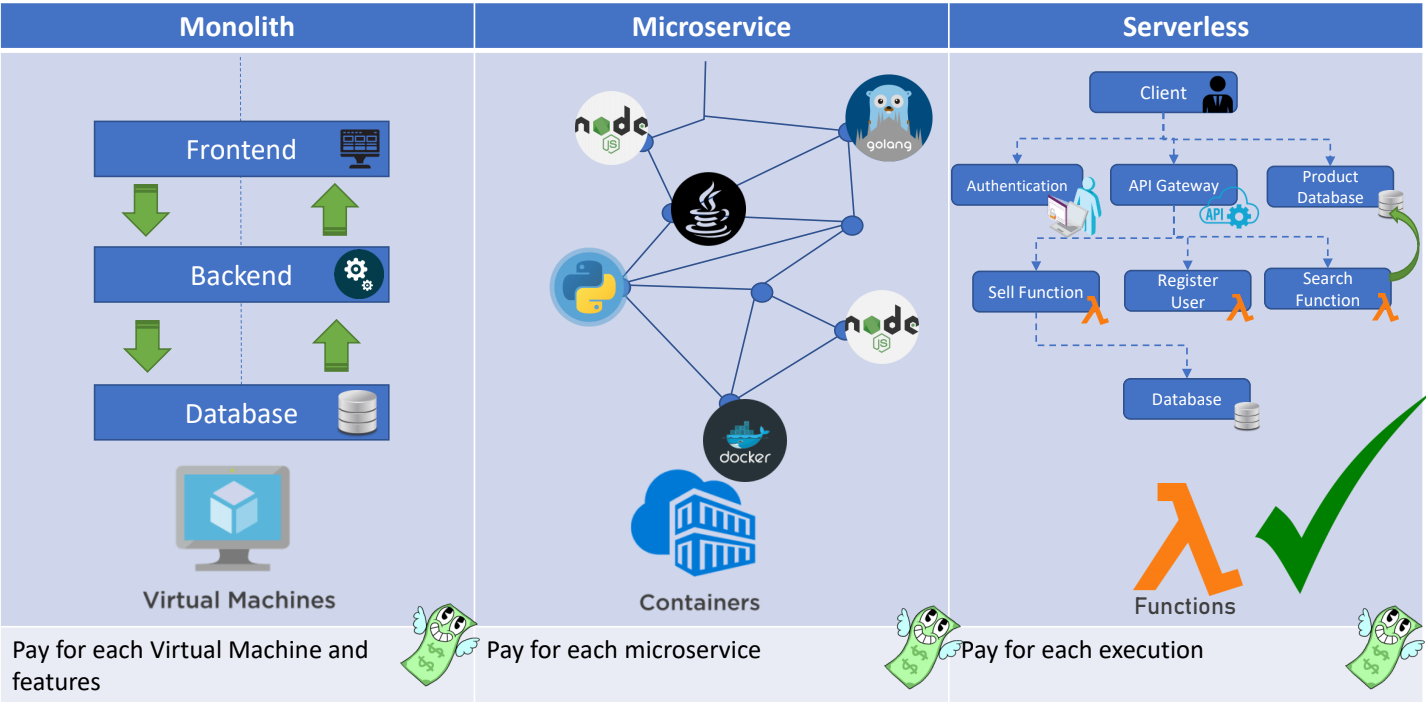
\includegraphics[width=\textwidth]{img/architectures.png}
  \caption{Software architecture generations.} \label{fig1}
  \end{figure}

\subsubsection{Serverless Function} 
In math, a function is a relation between a set of inputs and an allowed set of
outputs, with the idea that each input goes to a single output. However, in
computer science a function is defined as a unit of code that has a role into a
greater code structure, works on varius inputs that usually are variables and throws a concrete
output that are the result of process those variables. One of the main features that belongs to
functions is that are stateless, they are focused on inputs and result with a simple process
that does not require an state, in the moment the inputs get into the function are already generating an output.  
In serverless,  events such as messages or HTTP requests can trigger these functions. 
Also, each function scales independently and is stateless with a short duration \cite{Baird2016}.
% I am not a fan of that definition of a function in CS - Mario
% Explain a bit more the "Stateless" part - Mario 

\section{Proposed architecture}

The propose is an architecture that allows to process a simple population that
is divided into sub-populations distributing them to process in different ways
and then communicating each other with purpose of increase the possibility to
find the best fitness of a function. This architecture can accept the use of an
indeterminate number of algorithms, allowing an easy hybridation and continuous
adaptability for different problems.

This architecture consist in 3 nodes, they are explained on the next points:

\begin{itemize}
  \item Manager: 
  Here a population conformed by sub-populations is created and the architecture
  initialize parameters to run the algorithm. Every time a sub-population is created 
  triggers an event that sends the subpopulations to be stored in a file JSON of
  MongoDB (preventing to saturate the memory) and to a message queue that is
  directed to its subsequent processing in the “Receiver” section that is our
  cluster of functions (Faas), because each sub-population requires the execution
  of a different algorithm, there is a different channel in the web sockets for
  each type of algorithm that triggers its respective serverless function. Once
  a subpopulation is processed, it is returned and a selection is made for the
  sub-population migration. The migration selection is made by taking the
  population attribute of the subpopulation that was returned and the
  subpopulation that it have been selected among the best 2, it should be noted
  that the decision to identify the best from the 2 is made randomly. Once the
  selection is made, a Splitting Point Uniform crossing will be made. The 2 new
  subpopulations replace their self and are resent it back to their respective
  serverless function and this process is repeited until completing the number
  of assigned migrations for the multi-population \cite{Ma2019,Santander-jim2018}. Of course this whole process
  is performed asynchronously avoiding wait for all responses from serverless
  functions to perform a crossover or a update of the multi-population status
  \cite{Lovbjerg2001,Jimeno2019}. In the following figure you can see from
  illustrative way how the multi-population is composed.
\begin{figure}[htp]
  \centering
  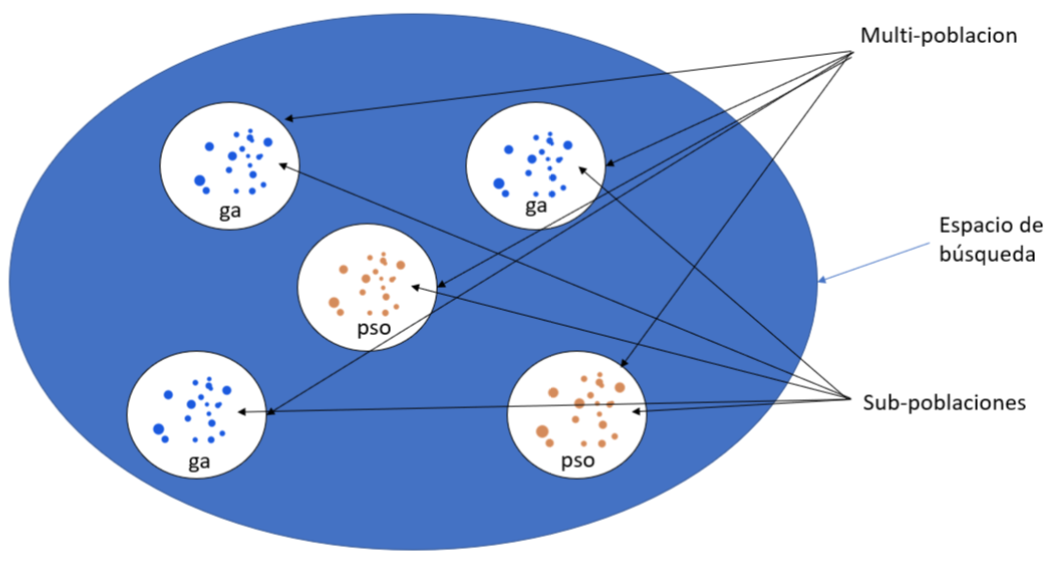
\includegraphics[width=0.7\textwidth]{img/multipopulation.png}
  \caption{Multipopulation representation.} \label{fig1}
  \end{figure}
  The mechanism to send the sub-population to the serverless functions is create a queue
  with a dimension of 2 positions that allow to compunicate in an asynchronous way.
\item Message Provider: Its purpose is the creation of a sub-population messages
queue which is the comunication channel between the sub-population Manager and
the Receiver (FaaS), each message is a trigger for the execution of a GA or PSO
function. Thanks to the message queue, it is possible to perform the serverless
functions asynchronously, avoiding that the algorithm wait for responses
independently of their duration and the simultaneous evaluation of different
sub-populations independent of its algorithm or characteristics.
\item Receiver: The following section contains the Serverless functions of the
algorithms to be executed, reduced the best possible using the functional
programming paradigm so that they can be converted into FaaS without problems,
in addition to achieving a completely clean and fast execution
\cite{Roberts2016} . Each message received on this node is executed in the form
of a multi-threaded process in parallel, this allows to having more than one
population-based search algorithm running at the same time, and making a copy of
itself each algorithm function as required.
\end{itemize}

To develop this architecture the applied technologies are based in JavaScript
using Node JS as it can be see it in the General Architecture Flowchart.

\begin{figure}[htp]
  \centering
  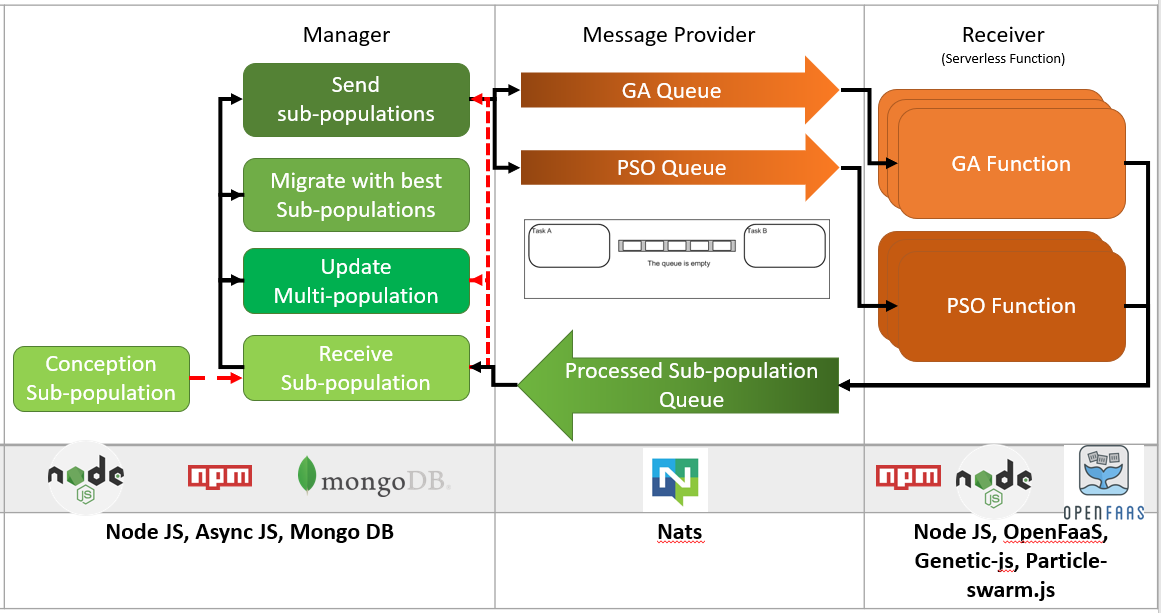
\includegraphics[width=0.9\textwidth]{img/general diagram architecture 2.png}
  \caption{General Architecture Flowchart.} \label{fig2}
  \end{figure}

\subsection{Sub-population definition}

Individuals are created composed of 2 types of information, the one that is
active or useful for crossing and the one that is not. The population contains
the series of possible solutions, while the rest contains the information on how
the processing for the search of the optimal solutions will be executed, linked
directly with their respective algorithms.

\begin{figure}[htp]
  \centering
  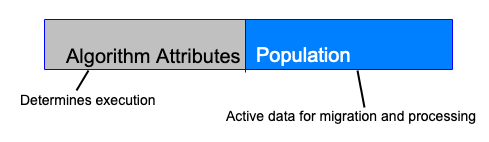
\includegraphics[width=0.6\textwidth]{img/subpopulationDefinition.png}
  \caption{Sub-population composition.} \label{fig3}
  \end{figure}

\subsection{Splitting Point Uniform Migration}

This architecture communicates sub-populations using migrations, taking information from 2 sub-populations and mixing them 
using a process similar to crossover in Genetic Algorithms, creating 2 completely new sub-populations
every time a processed sub-population arrives into the Manager node and replacing them self in the multi-population.

The migration created to this architecture is a method called Splitting Point Uniform that consist in a 
uniform mask that is created to apply the migration between individuals, vectors or both of them, from 2
sub-populations. The selected data are combined using the middle point between
the active values points by the binary mask generated randomly. This process iterates the 2 sub-populations to
randomly swap values and replace some of them with middle points \cite{Kramer2017,Kaya2011}.


\begin{figure}[htp]
  \centering
  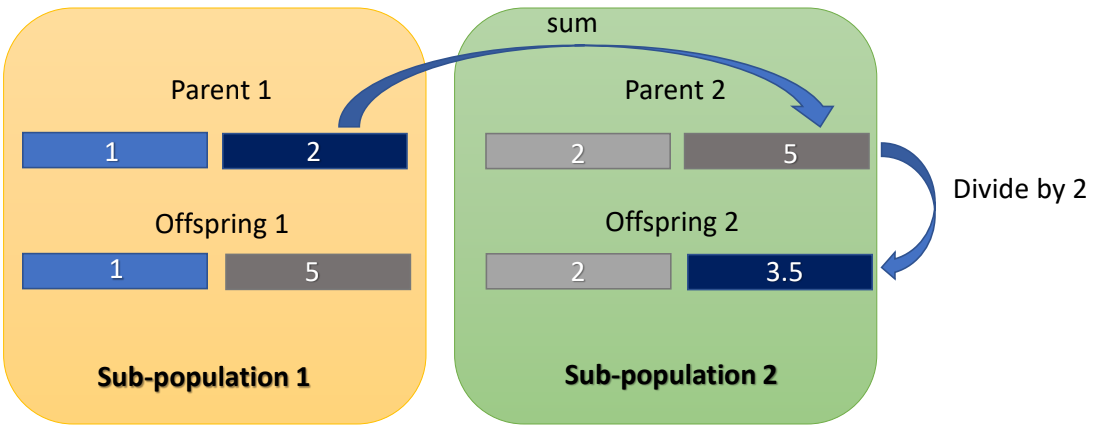
\includegraphics[width=0.9\textwidth]{img/splittinPointUniform.png}
  \caption{Splitting Point Uniform process.} \label{fig4}
  \end{figure}

  \subsection{Migration Selection} The 2 sub-populations selected to realize migration are one arrived sub-population from a serverless function and another one 
  using selection by tournament keeping up the information of the best
  sub-population of the multi-population but without discarding posible sub-populations that in a near future could be the clue to find optimal values.

\begin{figure}[htp]
  \centering
  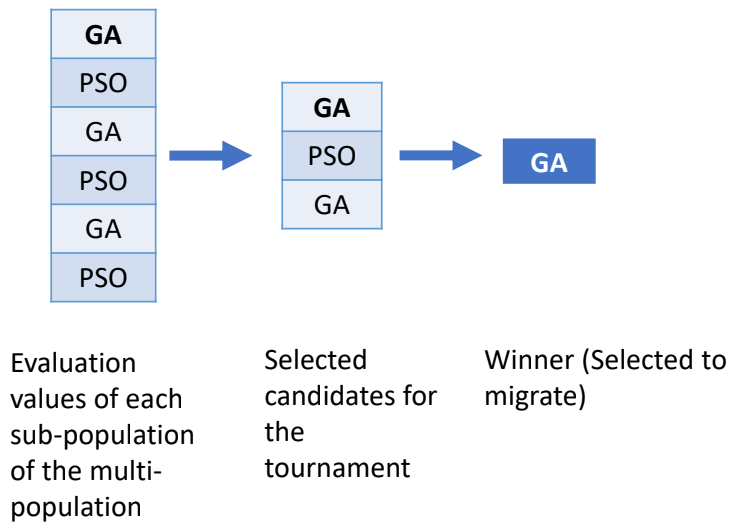
\includegraphics[width=0.5\textwidth]{img/selection.png}
  \caption{Selection by tournament.} \label{fig5}
  \end{figure}


\section{Experiments and Results}
\subsection{Experiments}
Now that an interaction between sub-populations with different algorithms it is
working and  hybridation have been a success, using until now the added
algorithms (GA and PSO) algorithms \cite{Kramer2017,Guerrero2017,Lalwani2019}, all thanks to the developed architecture,
lets procede to the experiments. This section is going to be the execution of
several experiments from 2 to 40 dimensions, with a stop criterial of an error
below  0.5E-8, without a parameter optimization method, waiting that the
architecture by its self would be enough to increase the possibility to find a
better optimal result than the traditional methods. All this hoping that the
results will probe the needness of this kind of architecture on increasing
dimensions. To test if the architecture was useful, several experiments were
made to solve benchmark functions, for this case the functions are Sphere,
Rastrigin and Rosenbrock. Using 10 sub-population for each experiment and
maximum 4 migrations per sub-population with different algorithms and parameters
for each sub-population.

\begin{figure}[htp]
  \centering
    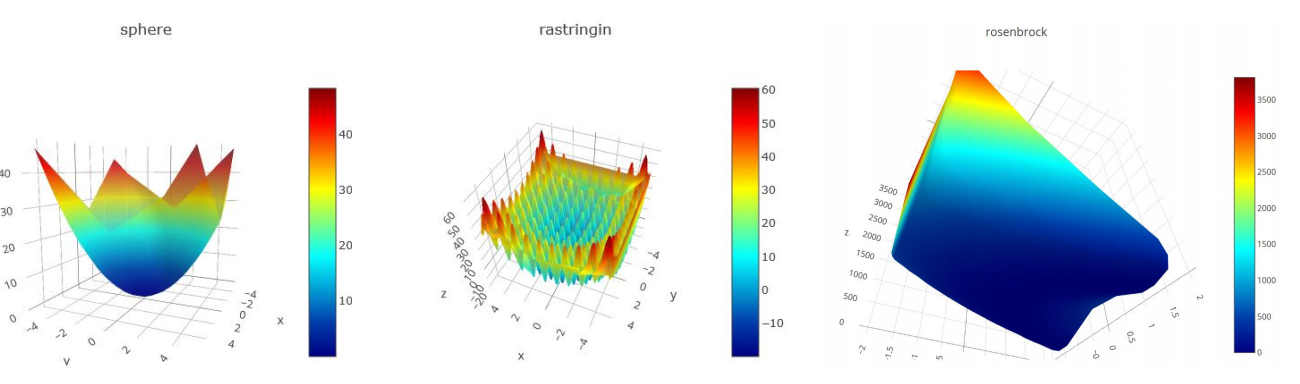
\includegraphics[width=0.7\textwidth]{img/benchmark.png}
    \caption{Benchmark functions for experimentation.} \label{fig6}
    \end{figure}

\subsection{Parameters Configuration} 

This architecture modifies the traditional way to work with population based
algorithms, then the experiments could not be parameterized as usually are.

Then the experiments are scaled by their number of evaluations and the
parameters must be configured to be adjusted to the next criterial, using the
next expression:

\begin{equation}
    \label{eq:hesitancy-interpretation}
   Evaluations = 10^{5} Dimensions
   \end{equation}

For example, if the experiment has 2 dimensions, the maximum number of
evaluations will be 200,0000, for 10 dimensions will be 1,000,000 of evaluacions
and the same with the others dimensions.









   \begin{table}[htp]
    \caption{2 dimension parameters}
    \label{table:ga-pso-parameters-2}
    \centering
    \begin{tabular}{|l|l|}
    \hline
    Parameter & Value \\
    \hline
    \hline
    GA Optimization & Minimize \\
    \hline
    GA Generations & 50 \\
    \hline
    GA Dimensions & 2 \\
    \hline
    GA Population size & 100 \\
    \hline
    GA Mutation & Random(Tournament2,Tournament3,Random \\
    &  ,RandomLinearRank,Sequential,Fittest)\\
    \hline
    GA Crossover & Tournament3 \\
    \hline
    GA Crossover percentage & Random[10\%, 80\%] \\
    \hline
    GA Mutation percentage & Random[10\%,50\%] \\
    \hline
    GA Crossover function & Uniforme de punto medio \\
    \hline
    GA Mutation Function & gaussian \\
    \hline
    PSO Optimization & Minimiza \\
    \hline
    PSO Iterations & 50 \\
    \hline
    PSO Dimensions & 2 \\
    \hline
    PSO Vector size & 100 \\
    \hline
    PSO Social factor & Random[0.5,4.0] \\
    \hline
    PSO Individual factor & Random[0.5,4.0] \\
    \hline
    PSO Inercia factor & Random[0.5,4.0] \\
    \hline
    \end{tabular}
    \end{table}

\begin{figure}[htp]
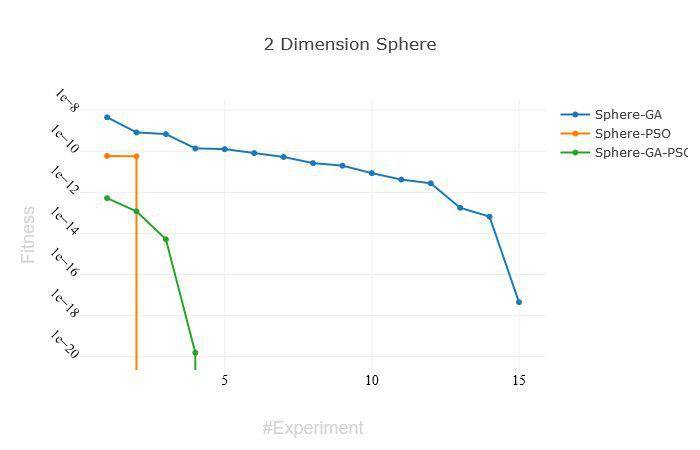
\includegraphics[width=\textwidth]{img/2-sphere.jpg}
\caption{2 dimension experiments Sphere.} \label{fig7}
\end{figure}

\begin{figure}[htp]
  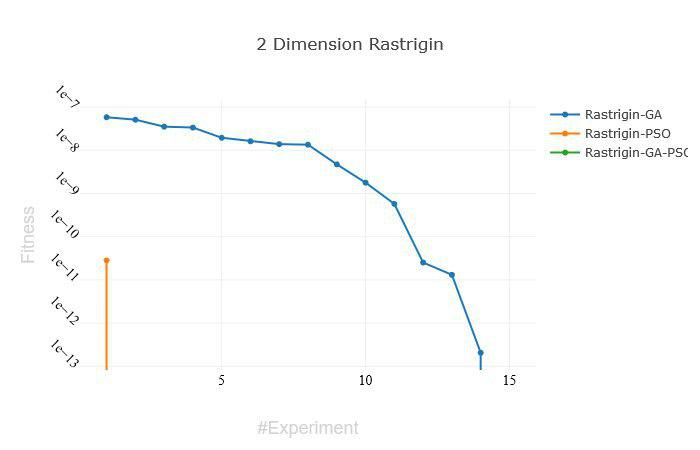
\includegraphics[width=\textwidth]{img/2-rastrigin.jpg}
  \caption{2 dimension experiments Rastrigin.} \label{fig8}
  \end{figure}
  
\begin{figure}[htp]
  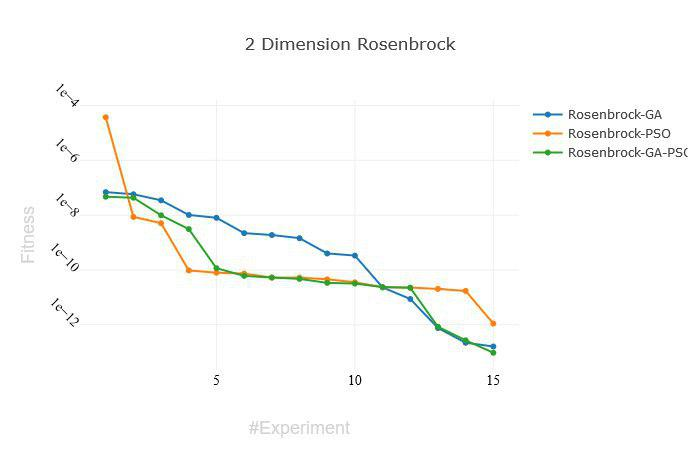
\includegraphics[width=\textwidth]{img/2-rosenbrock.jpg}
  \caption{2 dimension experiments Rosenbrock.} \label{fig9}
  \end{figure}

\begin{table}[htp]
    \caption{2 dimensional experiment results}
    \label{table:resultados-2}
    \centering
    \begin{tabular}{|c|c|c|c|}
    \hline
    Fn & Best & AVG & Experiment Number \\
    \hline
    \hline
    Rastrigin GA & 0 & 1.65377E-08 & 15\\
    \hline
    Rastrigin PSO & 0 & 1.8872E-12 & 15\\
    \hline
    Rastrigin GA-PSO & 0 & 0 & 15\\
    \hline
    Sphere GA & 4.53222E-18 & 4.36977E-10 & 15\\
    \hline
    Sphere PSO & 0 & 7.8012E-12 & 15\\
    \hline
    Sphere GA-PSO & 0 & 4.33161E-14 & 15\\
    \hline
    Rosenbrock GA & 1.62335E-13 & 1.24176E-08 & 15\\
    \hline
    Rosenbrock PSO & 1.11674E-12 & 2.47795E-06 & 15\\
    \hline
    Rosenbrock GA-PSO & 9.5809E-14 & 6.90695E-09 & 15\\
    \hline
    \end{tabular}
    \end{table}
  
    \begin{table}[htp]
      \caption{10 dimensions parameters}
      \label{table:ga-pso-parameters-10}
      \centering
      \begin{tabular}{|l|l|}
      \hline
      Parameter & Value \\
      \hline
      \hline
      GA Optimization & Minimiza \\
      \hline
GA Generations & 70 \\
      \hline
GA Dimensions & 10 \\
      \hline
GA Population size & 200 \\
      \hline
GA Mutation & Random(Tournament2,Tournament3,Random \\
      &  ,RandomLinearRank,Sequential,Fittest)\\
      \hline
GA Crossover \\
      \hline
GA Crossover percentage & Random[10\%, 80\%] \\
      \hline
GA Mutation percentage & Random[10\%,50\%] \\
      \hline
GA Crossover function & Uniforme de punto medio \\
      \hline
GA Mutation Function & gaussian \\
      \hline
PSO Optimization & Minimiza \\
      \hline
PSO Iterations & 70 \\
      \hline
PSO Dimensions & 10 \\
      \hline
PSO Vector size & 200 \\
      \hline
PSO Social factor & Random[0.5,4.0] \\
      \hline
PSO Individual factor & Random[0.5,4.0] \\
      \hline
PSO Inercia factor & Random[0.5,4.0] \\
      \hline
      \end{tabular}
      \end{table}
    
      \begin{figure}[htp]
        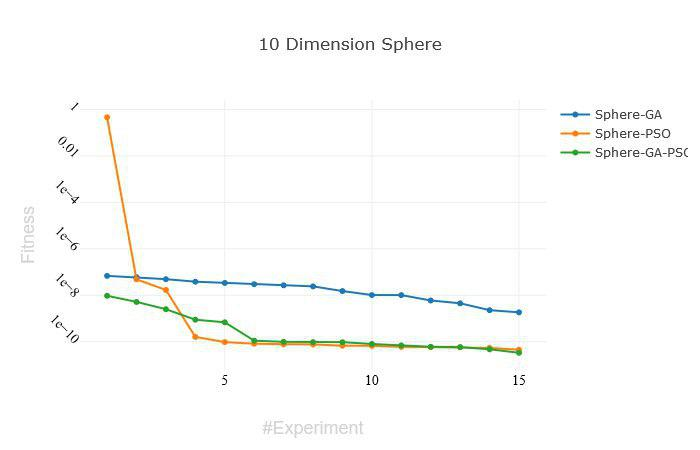
\includegraphics[width=\textwidth]{img/10-sphere.jpg}
        \caption{10 dimensions experiments Sphere.} \label{fig10}
        \end{figure}

        \begin{figure}[htp]
          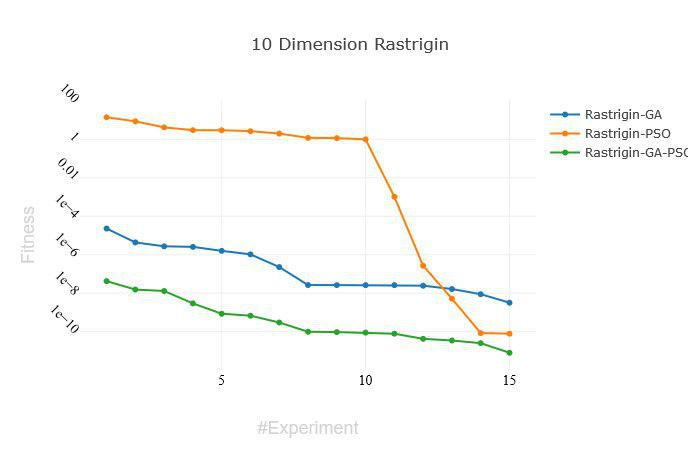
\includegraphics[width=\textwidth]{img/10-rastrigin.jpg}
          \caption{10 dimensions experiments Rastrigin.} \label{fig11}
          \end{figure}

          \begin{figure}[htp]
            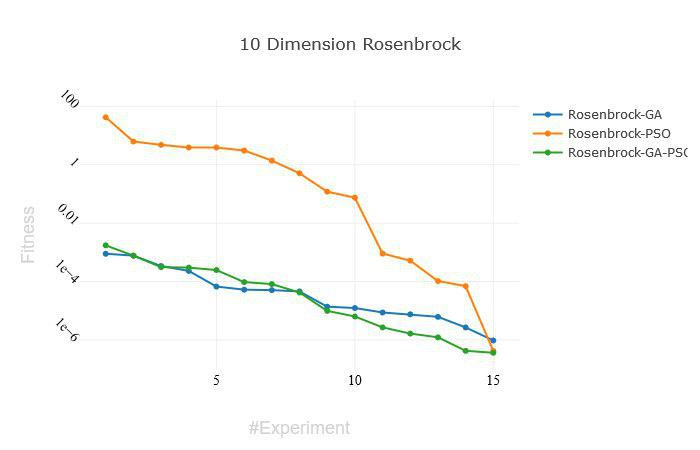
\includegraphics[width=\textwidth]{img/10-rosenbrock.jpg}
            \caption{10 dimensions experiments Rosenbrock.} \label{fig12}
            \end{figure}

        \begin{table}[htp]
          \caption{10 dimensional experiment results}
          \label{table:resultados-2}
          \centering
          \begin{tabular}{|l|l|l|l|}
          \hline
          Fn & Best & Average & Experiment Number \\
          \hline
          \hline
          Rastrigin GA & 3.21768E-09 & 2.38015E-06 & 15\\
          \hline
          Rastrigin PSO & 7.8586E-11 & 2.715716161 & 15\\
          \hline
          Rastrigin GA-PSO & 8.01492E-12 & 5.08668E-09 & 15\\
          \hline
          Sphere GA & 1.84051E-09 & 2.5389E-08 & 15\\
          \hline
          Sphere PSO & 4.50351E-11 & 4.72855E-09 & 15\\
          \hline
          Sphere GA-PSO & 3.33851E-11 & 1.30062E-09 & 15\\
          \hline
          Rosenbrock GA & 9.58323E-07 & 1.24176E-08 & 15\\
          \hline
          Rosenbrock PSO & 4.16711E-07 & 4.431565444 & 15\\
          \hline
          Rosenbrock GA-PSO & 3.62472E-07 & 0.000240251 & 15\\
          \hline
          \end{tabular}
          \end{table}

          \begin{table}[htp]
            \caption{Parametros experimentos 20 dimensiones}
            \label{table:ga-pso-parameters-20}
            \centering
            \begin{tabular}{|l|l|}
            \hline
            Parameter & Value \\
            \hline
            \hline
            GA Optimization & Minimiza \\
            \hline
            GA Generations & 70 \\
            \hline
            GA Dimensions & 20 \\
            \hline
            GA Population size & 200 \\
            \hline
            GA Mutation & Random(Tournament2,Tournament3,Random \\
            &  ,RandomLinearRank,Sequential,Fittest)\\
            \hline
            GA Crossover & Tournament3 \\
            \hline
            GA Crossover percentage & Random[10\%, 80\%] \\
            \hline
            GA Mutation percentage & Random[10\%,50\%] \\
            \hline
            GA Crossover function & Uniforme de punto medio \\
            \hline
            GA Mutation Function & gaussian \\
            \hline
            PSO Optimization & Minimiza \\
            \hline
            PSO Iterations & 70 \\
            \hline
            PSO Dimensions & 20 \\
            \hline
            PSO Vector size & 200 \\
            \hline
            PSO Social factor & Random[0.5,4.0] \\
            \hline
            PSO Individual factor & Random[0.5,4.0] \\
            \hline
            PSO Inercia factor & Random[0.5,4.0] \\
            \hline
            \end{tabular}
            \end{table}
          
            \begin{figure}[htp]
              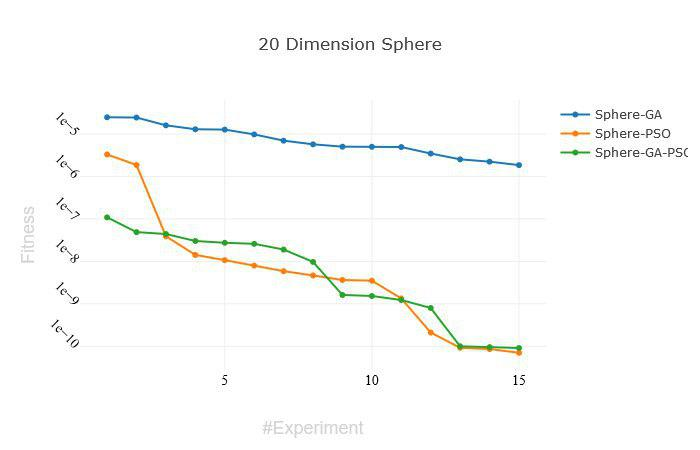
\includegraphics[width=\textwidth]{img/20-sphere.jpg}
              \caption{20 dimensions experiments Sphere.} \label{fig13}
              \end{figure}
      
              \begin{figure}[htp]
                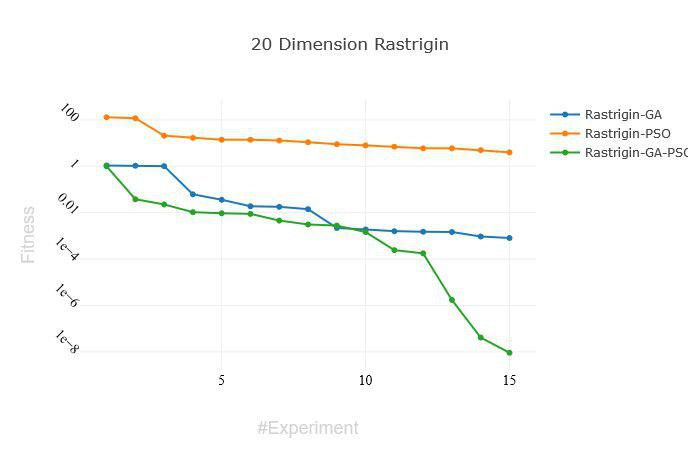
\includegraphics[width=\textwidth]{img/20-rastrigin.jpg}
                \caption{20 dimensions experiments Rastrigin.} \label{fig14}
                \end{figure}
      
                \begin{figure}[htp]
                  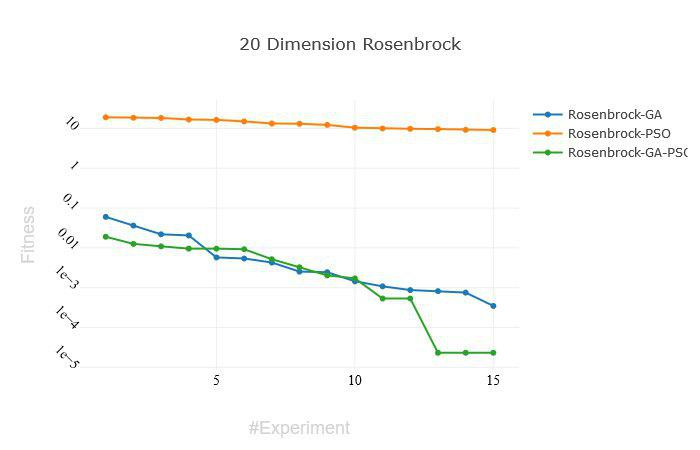
\includegraphics[width=\textwidth]{img/20-rosenbrock.jpg}
                  \caption{20 dimensions experiments Rosenbrock.} \label{fig15}
                  \end{figure}

                  \begin{table}[htp]

    \caption{Resultados 20 dimensiones}
    \label{table:resultados-2}
    \centering
    \begin{tabular}{|l|l|l|l|}
    \hline
    Fn & Best & Average & Experiment Number \\
    \hline
    \hline
    Rastrigin GA & 0.000808633 & 0.220596203 & 15\\
    \hline
    Rastrigin PSO & 3.988070734 & 25.51777514 & 15\\
    \hline
    Rastrigin GA-PSO & 9.13E-09 & 7.38E-02 & 15\\
    \hline
    Sphere GA & 1.84051E-09 & 9.22715E-06 & 15\\
    \hline
    Sphere PSO & 7.04E-11 & 3.50E-07 & 15\\
    \hline
    Sphere GA-PSO & 9.11E-11 & 2.13E-08 & 15\\
    \hline
    Rosenbrock GA & 0.000348015 & 0.010958941 & 15\\
    \hline
    Rosenbrock PSO & 9.119539342 & 13.37613983 & 15\\
    \hline
    Rosenbrock GA-PSO & 2.31663E-05 & 0.005608855 & 15\\
    \hline
    \end{tabular}
    \end{table}

    \begin{table}[htp]
      \caption{Parametros experimentos 40 dimensiones}
      \label{table:ga-pso-parameters-20}
      \centering
      \begin{tabular}{|c|c|}
      \hline
      Parameter & Value \\
      \hline
      \hline
      GA Optimization& Minimiza \\
      \hline
      GA Generations & 70 \\
      \hline
      GA Dimensions & 40 \\
      \hline
      GA Population size & 200 \\
      \hline
      GA Mutation & Random(Tournament2,Tournament3,Random \\
      &  ,RandomLinearRank,Sequential,Fittest)\\
      \hline
      GA Crossover \\
      \hline
      GA Crossover percentage & Random[10\%, 80\%] \\
      \hline
      GA Mutation percentage & Random[10\%,50\%] \\
      \hline
      GA Crossover function & Uniforme de punto medio \\
      \hline
      GA Mutation Function & gaussian \\
      \hline
      PSO Optimization & Minimiza \\
      \hline
      PSO Iterations & 70 \\
      \hline
      PSO Dimensions & 40 \\
      \hline
      PSO Vector size& 200 \\
      \hline
      PSO Social factor & Random[0.5,4.0] \\
      \hline
      PSO Individual factor & Random[0.5,4.0] \\
      \hline
      PSO Inercia factor & Random[0.5,4.0] \\
      \hline
      \end{tabular}
      \end{table}
    
      \begin{figure}[htp]
        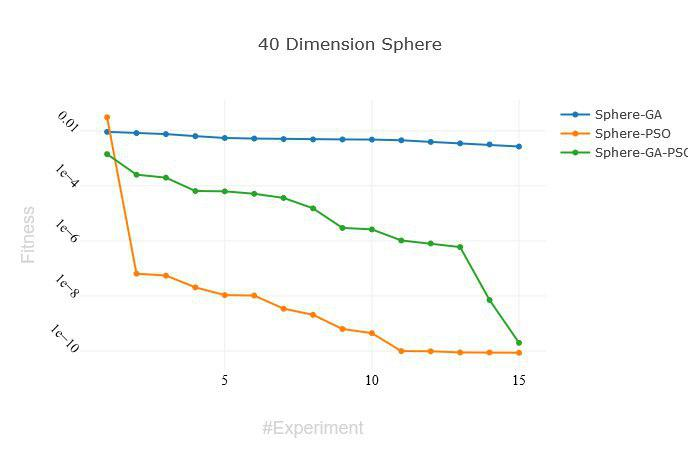
\includegraphics[width=\textwidth]{img/40-sphere.jpg}
        \caption{40 dimensions experiments Sphere.} \label{fig1}
        \end{figure}

        \begin{figure}[htp]
          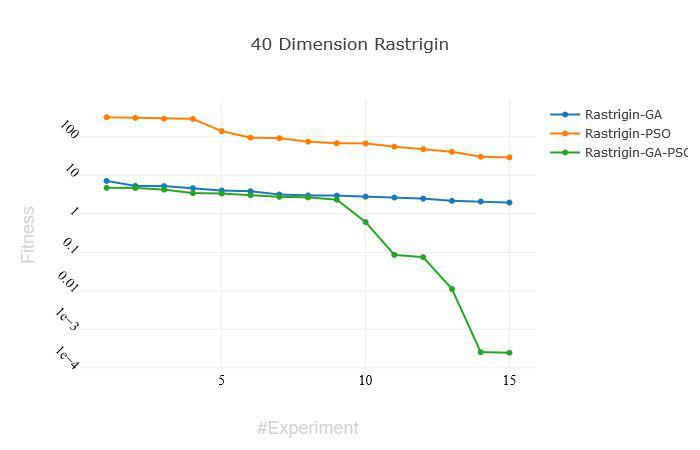
\includegraphics[width=\textwidth]{img/40-rastrigin.jpg}
          \caption{40 dimensions experiments Rastrigin.} \label{fig1}
          \end{figure}

          \begin{figure}[htp]
            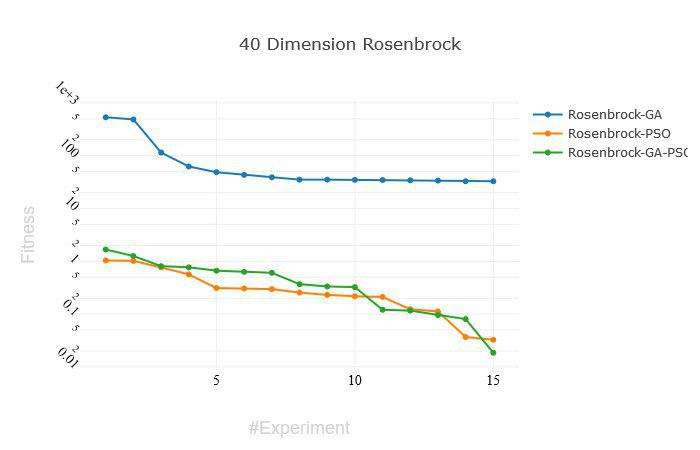
\includegraphics[width=\textwidth]{img/40-rosenbrock.jpg}
            \caption{40 dimensions experiments Rosenbrock.} \label{fig1}
            \end{figure}

            \begin{table}[htp]
              \caption{Resultados 40 dimensiones}
              \label{table:resultados-2}
              \centering
              \begin{tabular}{|l|l|l|l|}
              \hline
              Fn & Best & Average & Experiment Number \\
              \hline
              \hline
              Rastrigin GA & 1.95478879 & 3.560837088 & 15\\
              \hline
              Rastrigin PSO & 29.06596132 & 130.2865863 & 15\\
              \hline
              Rastrigin GA-PSO & 2.46E-04 & 2.13E+00 & 15\\
              \hline
              Sphere GA & 0.002686956 & 0.005302951 & 15\\
              \hline
              Sphere PSO & 8.68E-11 & 2.07E-03 & 15\\
              \hline
              Sphere GA-PSO & 2.00E-10 & 1.41E-04 & 15\\
              \hline
              Rosenbrock GA & 0.000348015 & 106.9287542 & 15\\
              \hline
              Rosenbrock PSO & 0.032708559 & 0.368395353 & 15\\
              \hline
              Rosenbrock GA-PSO & 0.018538924 & 0.525086565 & 15\\
              \hline
              \end{tabular}
              \end{table}
% ---- Bibliography ----
%
% BibTeX users should specify bibliography style 'splncs04'.
% References will then be sorted and formatted in the correct style.
%
% \bibliographystyle{splncs04}
% \bibliography{mybibliography}
%
\section{Conclusion}

This architecture is completely scalable and useful for hybridation of multiple algorithms,
until now is only GA and PSO but according with the results with this kind of architecture
there is no limit and it works better than multi-populations with only one algorithm, also
every experiment executes in short times because serverless functions searching in an asynchronous way getting a fast convergence.

\section{Future work}

To get a continuous improvement it is believed that it is required a sort of mutation applied to the 
sub-populations. This mutation would be a swapping type, taking the algoritm parameters from the best and the worst 
sub-populations, increasing the possibilities to get and optimal result, preventing get stucked into a local optimum.
Of course it is expected to use this architecture using more algorithms than GA and PSO.


\bibliography{samplepaper}
      \bibliographystyle{ieeetr}
  
\end{document}
